\documentclass[DM,lsstdraft,toc,usenatbib]{lsstdoc}

% Package imports go here
\usepackage{amsmath}	% Advanced maths commands
\usepackage{amssymb}
\usepackage{gensymb}  % degree symbol 
\usepackage{natbib}  % bibliography
\usepackage{cprotect} 
% Local commands go here

%% Journal abbreviations
%\bibliographystyle{aasjournal}

\title[Crowded fields ]{LSST  Crowded Fields photometry}

\author{
K.~Suberlak, C.~Slater,
\v{Z}.~Ivezi\'c, P.~Yoachim}

\setDocRef{LSST-2017}
\date{\today}
\setDocRevision{TBD}
\setDocStatus{draft}
\setDocAbstract{%
A report the status of crowded field photometry. We evaluate the need for performing better photometry in crowded fields by quantifying areas of the sky at a given density level. We provide an overview of density metrics, photometric methods applicable in a given stellar density regime, and recommendations for areas of improvement in the LSST Stack.}

% Change history defined here. Will be inserted into
% correct place with \maketitle
% OLDEST FIRST: VERSION, DATE, DESCRIPTION, OWNER NAME
\setDocChangeRecord{%
\addtohist{1}{2017-07-16}{First draft.}{Krzysztof Suberlak}
\addtohist{2}{2017-10-19}{Major edits.}{Krzysztof Suberlak}
}

\begin{document}

% Create the title page
% Table of contents will be added automatically if "toc" class option
% is used.
\maketitle

\section{Introduction}

This is a document to report on quantifying the performance expectations and options with respect to crowded field processing.

The Large Scale Synoptic Telescope (LSST) will sample very diverse regions when it comes to stellar density, or crowdedness : from high density low-galactic latitude regions that have tens of millions of sources per square degree, to low-density regions towards the galactic poles with less than thousand sources per square degree. 

As mentioned by ~\cite{bosch2017} with regards to Hyper Suprime CAM software pipeline (based on LSST Stack, which in turn builds on the experience of the SDSS  Photo pipeline), deblending and performing a successful photometry is an inherent part of any astronomical data processing pipeline. The boundaries between deblending, measurement and detection blur in very high stellar densities, and the deeper the survey, the higher the stellar densities that it can encounter (see Sec 4.8.3 in \cite{bosch2017}). 

The way in which measurements may be affected by the crowdiness have been studied before - pilot study by ~\citep{hogg2001} confirmed the '30 beams per source' rule of thumb, albeit it depends on the source number counts (with steeper number counts we need more beams per source ). Following on that exploratory study,  ~\cite{olsen2003} describes more quantitative framework to address this issue in the era of large telescopes. 


\section{Identifying density regions}
We start with the LSST  Metrics Analysis Framework \footnote{\url{https://www.lsst.org/scientists/simulations/maf}} simulated stellar density map \footnote{\url{https://github.com/lsst/sims_maf}}, made with \verb|sims_maf/python/lsst/sims/maf/maps/createStarDensitymap.py|\footnote{\url{https://github.com/lsst/sims_maf/blob/a9bc8f6d00fae5d7ce4ff6ea7279d5a0fca29437/python/lsst/sims/maf/maps/createStarDensitymap.py}} by Peter Yoachim and Lynne Jones at UW. The dataset \verb|starDensity_r_nside_64.npz| contains 64 magnitude bins, and 49152  healpixels \footnote{see http://healpix.sourceforge.net for documentation of HEALPix}. Each pixel contains information about number of stars per square degree in a given magnitude bin.  

% WHY Southern Hemisphere  ?  
Using this data, we select magnitude bins smaller than r=24.5 in the Southern Hemisphere ($\delta < 0$).  We add stellar count across magnitude bins (selecting only  r <= 24.5 bins).   For each pixel we calculate the number of pixels that have a higher stellar count.  Since each pixel in HEALPix has an equal area, the fraction of pixel number above a certain threshold corresponds to the fraction of sky area above given density limit. See Fig.~\ref{fig:illustrate_density} for an illustration of how we define the stellar density - it is akin to a cumulative distribution. Therefore 'top 1\%' density means that only 1 in 100 pixels has a higher density than a given pixel.  Likewise,  'top 10\%' means that '10 \%' of pixels in the selected hemisphere have higher density. 

\begin{figure}
\includegraphics[width=1.0\columnwidth]{figs/Southern_sky_r_lt245_twiny.png}
%\vskip -0.15in
\caption{Illustration of how the stellar density is quantified in terms of relative pixel density. We express stellar density both in terms of number of stars per square degree (bottom axis), as well as in terms of product of sources per square arcsecond and psf effective area (upper axis )}
\label{fig:illustrate_density}
\end{figure} 


Since this definition of density includes all pixels that are within 'top 20\%', we take selection around the percentiles so that :

\begin{itemize}
\item top  1 \%  means  fraction of sky with greater density is 0.01
\item 5 \% region means such that between  4\% and 6\%
\item 20 \% region  includes   19\% - 21\%
\item 50 \% region includes 49\% - 51\% 
\end{itemize}


We illustrate the location of pixels representative of these density brackets on the sky in various projections  and coordinate systems :  cylindrical (Mercator) projection  in equatorial coordinates on Fig.~\ref{fig:cart_equat},  Mollweide projection in equatorial coordinates on Fig.~\ref{fig:mollw_equat},  and the same in galactic coordinates on Fig.~\ref{fig:mollw_galactic}. 


\begin{figure}
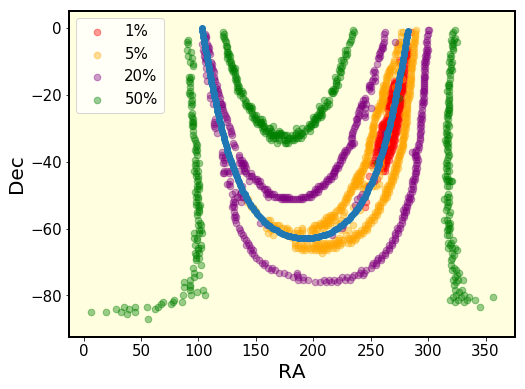
\includegraphics[width=1.0\columnwidth]{figs/Illustrate_density_regions.png}
%\vskip -0.15in
\caption{Illustration of location of regions representative of different relative density in cylindrical projection, equatorial coordinates. The blue solid line marks the location of Galactic equator. }
\label{fig:cart_equat}
\end{figure} 



\begin{figure}
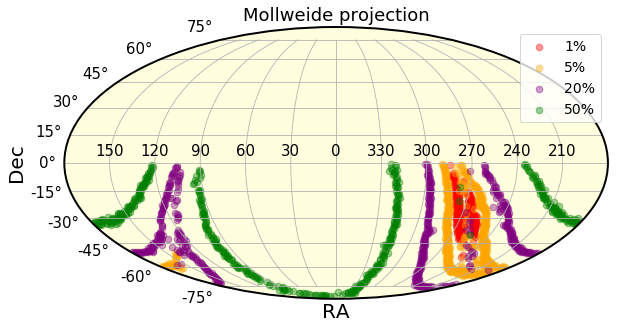
\includegraphics[width=1.0\columnwidth]{figs/Illustrate_density_regions_mollw.png}
%\vskip -0.15in
\caption{Same as Fig.~\ref{fig:cart_equat}, but in Mollweide projection, with Equatorial coordinates.}
\label{fig:mollw_equat}
\end{figure} 



\begin{figure}
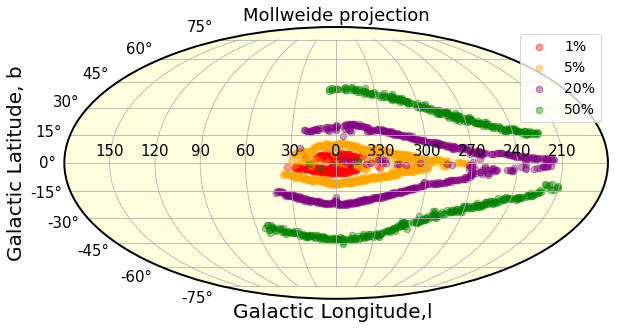
\includegraphics[width=1.0\columnwidth]{figs/Illustrate_density_regions_mollw_galactic.png}
%\vskip -0.15in
\caption{Same as Fig.~\ref{fig:mollw_equat}, but in Galactic coordinates, which emphasizes the location of regions representing different density with regards to the Milky Way. It makes sense that the highest density regions in the Southern Hemisphere ($\delta < 0$) are located close to the galactic bulge, and the decreasing density regions approximately trace the shape of our galaxy.}
\label{fig:mollw_galactic}
\end{figure} 

\section{DECam images for fields representative of given source density }

We compare the MAF estimates of stellar density in various density regimes to Dark Energy Camera (DECam)  data, taken with the 4-m Cerro Tololo Inter-American Observatory telescope (CTIO)\footnote{see \url{http://www.ctio.noao.edu/noao/node/1033}}. To circumvent lack of possibiliy of querying by a list of coordinates  at the NOAO Data Archive \footnote{\url{http://archive.noao.edu/search/query}}, we used the SQL query.  We first obtained all data that fulfilled very loose criteria:
\begin{itemize}
\item telescope = 'ct4m'
\item instrument = 'decam'
\item 90 sec < exposure < 125 sec 
\item release\_date < ‘2017-07-24'
\item dec < 0 
\item proctype = 'InstCal' 
\item prodtype = 'image'
\item filter is  u, g, r,  or VR 
\end{itemize}
(the exact SQL query used is available in the Appendix ~\ref{sec:sql_noao_decam}). The exposure time was chosen to match the LSST depth at 30 second exposure.

We obtained 11928 rows (individual fields) fulfilling these criteria. The location of these observations on the sky, with overlaid MAF density regions, is shown on Fig.~\ref{fig:decam_regions}. 

 
\begin{figure}
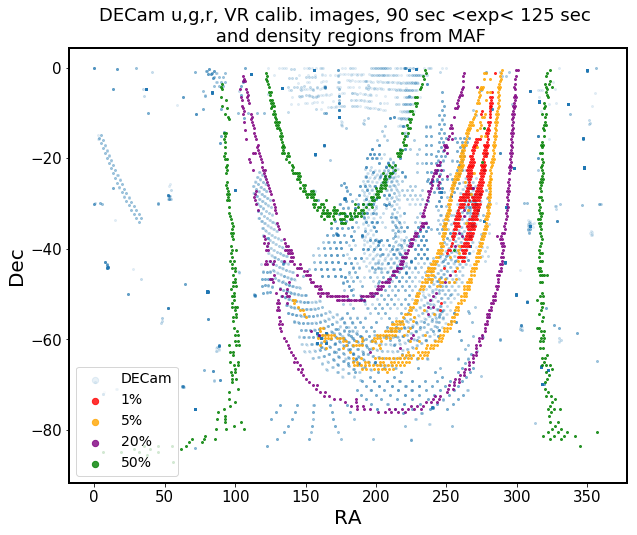
\includegraphics[width=1.0\columnwidth]{figs/Illustrate_density_regions_DECam.png}
%\vskip -0.15in
\caption{DECam observations with exposure $\in [90,125] $ sec, $\delta < 0$, taken in  u,g,r, or VR filter.  }
\label{fig:decam_regions}
\end{figure} 

We used AstroPy SkyCoord package to match the coordinates of MAF healpixels to DECam imaging data. For instance, of the 244 healpixels in the top 1\% density regime  91 had a DECam counterpart within 30 arcminutes.  We allowed very liberal bounds to only approximately point at the same region of the sky - see Fig.~\ref{fig:decam_matches_top}. 

\begin{figure}
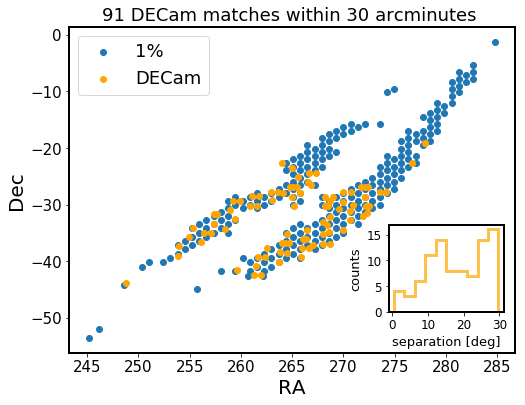
\includegraphics[width=1.0\columnwidth]{figs/Illustrate_top_1_perc_DECam_matches.png}
%\vskip -0.15in
\caption{DECam observations with exposure $\in [90,125] $ sec, $\delta < 0$, taken in  u,g,r, or VR filter, matched using 2D separation to MAF healpixels within the highest stellar density bins. The inset shows the distribution of separation between healpix coordinates and DECam image center. Each DECam image is a mosaic of CCDs, and each mosaic element covers approximately 9x18 arcminutes (see Fig.~\ref{fig:decam_mosaic_ccd} for illustration). }
\label{fig:decam_matches_top}
\end{figure} 


\begin{figure}
\includegraphics[width=1.0\columnwidth]{figs/Fig_4-3_NOAO_DECam_ccd_mosaic.png}
%\vskip -0.15in
\caption{An illustration of the DECam CCD mosaic image plane, adapted from ~\citep{shaw2015}, Fig.4-3. The color corresponds to the one of the four sets of read-out electronics (orange,pink, blue,yellow), or the guiding (green) and focus (magenta) CCDS.  The grey CCDs do not function properly. In using the LSST Stack processing we used CCD10 (S22)  or CCD11 (S23) (for astrometric comparison).   }
\label{fig:decam_mosaic_ccd}
\end{figure} 

\subsection{DAOStarFinder source detection}
Per each density regime, we selected five random DECam fields, and performed source extraction with DAOStarFinder\footnote{\url{http://photutils.readthedocs.io/en/stable/photutils/detection.html}}.  This tool uses a classic DAOFIND algorithm~\citep{stetson1987}, and  we used it to verify the plausibility of the MAF source densities using real data.  DECam employs mosaic CCDs - each  field, which can be downloaded as a fits.fz compressed file, is split into 60 primary HDUs. FITS viewing software, such as ds9, by default open the first element (HDU[1]), and we decided to perform source extraction on this one element of the mosaic per field, since each element is of the same size, and is equally representative of the field. The size of each element of the mosaic is 2046x4094 pixels, with pixel scale of 0.27 arcsec / px , so that a single mosaic element covers an area of 0.047117 sq.deg. Using the FWHM information from the FITS header, and sigma clipped standard deviation $\sigma$, we performed source extraction with the detection threshold at $5 \sigma$ level, setting the detection threshold at $5\sigma$, and scaled it up to the source count per square degree to allow comparison with MAF data.  

\subsection{TRILEGAL queries}
We also  obtained TRILEGAL\footnote{\url{http://stev.oapd.inaf.it/cgi-bin/trilegal}} simulation results for each of the DECam fields, submitting to the online form the DECam ra,dec, and field size (using the size of a single mosaic element, as for DAOStarFinder source extraction -  approximately 0.047117 sq.deg. per field ). We limited the query results selecting r < 24.5 with  LSST ugrizy photometric system, keeping all other settings as default.  


\subsection{Comparison of MAF, DAOStarFinder, and TRILEGAL counts}
We used the number of sources per TRILEGAL output file, and scaled it to the degree level to compare with MAF and DAO.  The results are shown in Tables ~\ref{tab:one_perc}, ~\ref{tab:five_perc} ,~\ref{tab:twenty_perc} ,~\ref{tab:fifty_perc} for 1\%,5\%,20\% and 50 \% density levels. 


% 1 percent 

\begin{table}
\begin{tabular}{cccccc}
archive & l & b & TRILEGAL & MAF & DAO \\
c4d\_140624\_080728\_ooi\_r & 13.70 & -4.43 & 7,960,511 & 2,650,680 & 498,760 \\
c4d\_170428\_094150\_ooi\_g & 356.86 & -3.90 & 39,852,793 & 4,587,804 & 375,980 \\
c4d\_170501\_055757\_ooi\_g & 356.26 & 5.05 & 16,352,821 & 2,659,968 & 285,630 \\
c4d\_170504\_084722\_ooi\_g & 4.26 & 5.15 & 15,586,874 & 2,833,740 & 561,795 \\
\end{tabular}
\caption{Source density comparison for 1\% density level : TRILEGAL, DAO and MAF columns contain stellar counts from TRILEGAL simulation , DAOStarFinder based on DECam data, and MAF simulation, respectively. Simulation results are  limited by LSST r < 24.5. All counts are in stars per square degree. }
\label{tab:one_perc}
\end{table}
 

% images of 1 and 5 percent regions 
\begin{figure}
\begin{minipage}[t]{0.5\linewidth}
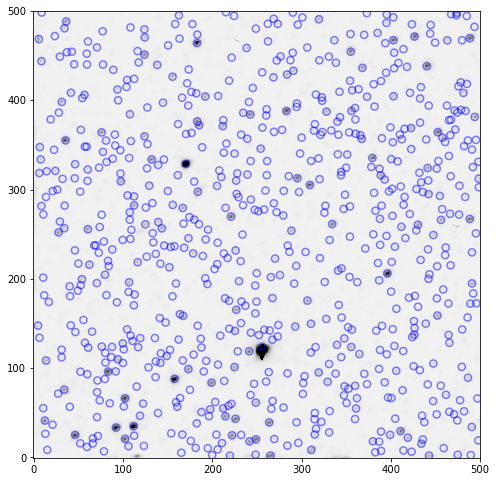
\includegraphics[width=\linewidth]{figs/c4d_170504_084722_ooi_g_v1_1_sub_500px.png}
\caption{500x500 pixels (135x135 arcseconds)  subregion of DECam field c4d\_170504\_084722\_ooi\_g,
a top 1\% density region. With DAOPhot threshold set at 5 $\sigma$,  we detected 722 sources in this postage stamp miniature, corresponding to the area of 0.001406 sq degrees, which translates to 513,422 sources per square degree. At the same coordinates, MAF density is 2,833,740 sources per square degree, and TRILEGAL density is 15,586,874 sources per square degree. }
\label{fig:decam_1_perc_miniature}
\end{minipage}
\hfill
\begin{minipage}[t]{0.5\linewidth}
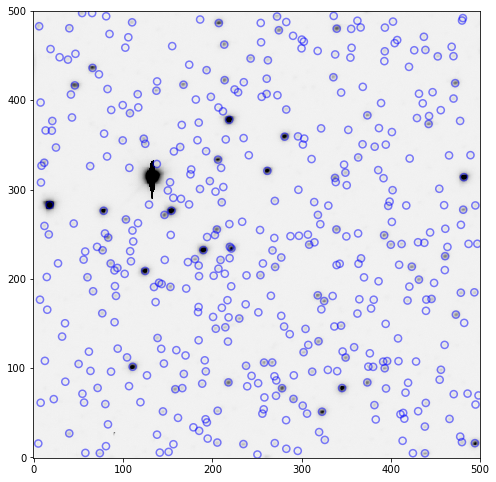
\includegraphics[width=\linewidth]{figs/c4d_170429_035748_ooi_g_v1_1_sub_500px.png}
\caption{500x500 pixels (135x135 arcseconds) subregion of DECam field c4d\_170429\_035748\_ooi\_g,  with 436  detected sources, in the 5 \% density region. The same DAOPhot settings as Fig.~\ref{fig:decam_1_perc_miniature}. That many sources in an area of 0.001406 sq degrees,  translates to 310,044 sources per square degree. At the same coordinates, MAF density is 807,156 sources per square degree, and TRILEGAL density is 1,870,414 sources per square degree. }
\label{fig:decam_5_perc_miniature}
\end{minipage}%
\end{figure}




% 5 percent

\begin{table}
\begin{tabular}{cccccc}
archive & l & b & TRILEGAL & MAF & DAO \\
c4d\_160316\_065235\_ooi\_g & 301.42 & 3.40 & 1,606,135 & 591,336 & 179,277 \\
c4d\_160825\_231905\_ooi\_g & 314.05 & 3.08 & 2,564,964 & 589,572 & 127,088 \\
c4d\_170429\_035748\_ooi\_g & 310.43 & -4.02 & 1,870,414 & 807,156 & 327,483 \\
tu1677011 & 4.48 & 8.70 & 2,530,163 & 810,144 & 509,093 \\
\end{tabular}
\caption{Source density comparison for 5\% density level, all columns and units as in Table ~\ref{tab:one_perc}}
\label{tab:five_perc}
\end{table}



% 21 percent 
\begin{table}
\begin{tabular}{cccccc}
archive & l & b & TRILEGAL & MAF & DAO \\
c4d\_170122\_055542\_ooi\_g & 242.43 & 3.77 & 341,343 & 116,856 & 66,282 \\
tu1661798 & 351.66 & 20.42 & 183,778 & 118,188 & 44,216 \\
tu1668579 & 217.04 & 1.21 & 379,319 & 111,096 & 54,004 \\
tu2187073 & 312.84 & 14.64 & 184,583 & 107,784 & 60,678 \\
\end{tabular}
\caption{Source density comparison for 20\% density level, all columns and units as in Table ~\ref{tab:one_perc}}
\label{tab:twenty_perc}
\end{table}

% images of 21 and 51 percent regions 

\begin{figure}
\begin{minipage}[t]{0.5\linewidth}
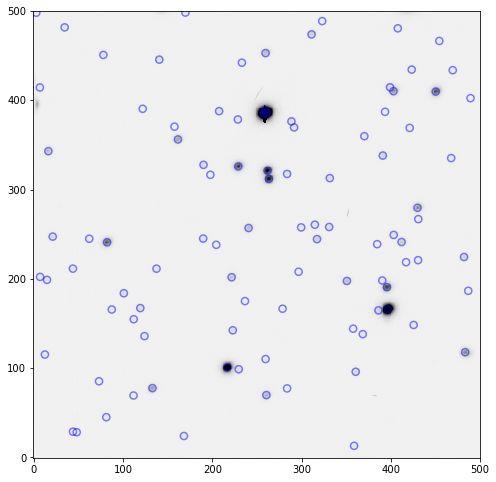
\includegraphics[width=\linewidth]{figs/c4d_170122_055542_ooi_g_v1_1_sub_500px.png}
\caption{500x500 pixels (135x135 arcseconds) subregion of DECam field c4d\_170122\_055542\_ooi\_g,  with 98  detected sources, in the  20 \% density region. The same DAOPhot settings as Fig.~\ref{fig:decam_1_perc_miniature}. That many sources in an area of 0.001406 sq degrees,  translates to 69,688 sources per square degree. At the same coordinates,  MAF density is  116,856 sources per square degree, and TRILEGAL density is 341,343 sources per square degree. }
\label{fig:decam_20_perc_miniature}
\end{minipage}
\hfill
\begin{minipage}[t]{0.5\linewidth}
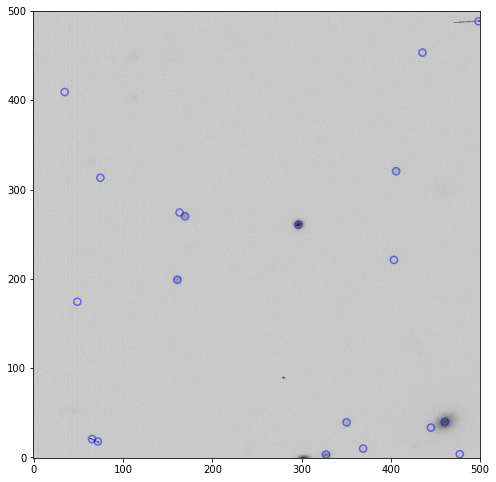
\includegraphics[width=\linewidth]{figs/c4d_160607_025052_ooi_g_v1_1_sub_500px.png}
\caption{500x500 pixels (135x135 arcseconds) subregion of DECam field c4d\_160607\_025052\_ooi\_g,  with 19  detected sources, in the  50 \% density region. The same DAOPhot settings as Fig.~\ref{fig:decam_1_perc_miniature}. That many sources in an area of 0.001406 sq degrees,  translates to 13,511 sources per square degree. At the same coordinates, MAF density is  20,052 per square degree, and TRILEGAL density is 29,607 sources per square degree.}
\label{fig:decam_20_perc_miniature}
\end{minipage}%
\end{figure}


% 51 percent  
\begin{table}
\begin{tabular}{cccccc}
archive & l & b & TRILEGAL & MAF & DAO \\
c4d\_150615\_005257\_ooi\_g & 344.39 & 41.67 & 27,633 & 21,024 & 12,904 \\
c4d\_160607\_025052\_ooi\_g & 2.92 & 41.68 & 29,607 & 20,052 & 13,371 \\
c4d\_160825\_034122\_ooi\_g & 345.83 & 1.28 & 18,364,268 & 20,268 & 91,177 \\
tu2046406.fits.fz & 220.89 & -16.08 & 41,832 & 19,944 & 35,974 \\
\end{tabular}
\caption{Source density comparison for 50\% density level, all columns and units as in Table ~\ref{tab:one_perc}}
\label{tab:fifty_perc}
\end{table}



\section{Performance of the LSST Stack}
We conducted more detailed studies of the LSST Stack performance. For each case there is a source catalog considered as ground 'truth', and images at various stellar densities that were processed with the LSST Stack. 

We aim to answerr the following questions: 

\begin{itemize}
\item how does the completeness vs. magnitude curve depend on the input source density  (expressed in terms of the dimensionless parameter that takes seeing into account) ? 
\item how does the photometric error (rms for true minus measured mag) vs. mag curve   depend on the input source density?
\end{itemize}

\subsection{LSST Stack on DECam}
 First we compared the DECaPS individual image catalogs\footnote{\url{http://decaps.skymaps.info/}}, which were made using iterative source detection (see ~\cite{schlafly2017}), and the LSST source catalogs, based on the  DECAm images.

We chose DECam fields representative of 20\% , 5\%, and 1\% level stellar densites. Querying the NOAO Archive against the field coordinates and  exposure range we obtained instcal,  wtmap, and dqmask per field. Using the staging functionality of the public ftp we downloaded these files onto the NCSA lsst-dev01 machine.  We processed each image with \verb|obs_decam| tools, specifically \verb|ingestImagesDecam.py|, and \verb|processCcd.py|. We analyzed the source catalogs and calibrated images. Using the 20\% region in g filter, 96-sec exposure and r-filter 50 sec exposure we constructed CMD diagram to demonstrate the functionality of photometric accuracy.  We demonstrated astrometric accuracy by using the 20\% region 96-second exposure in r-filter, and processing CCD10 and CCD11 - there is no overlap in the position of detected sources along the CCD boundary, which confirms that there is no major problem with astrometry. 



\subsection{LSST Stack on StarFast }
Second, we employed the StarFast image simulator\footnote{\url{https://dmtn-012.lsst.io}}, that simulates the volume with randomly distributed known population of stars. We simulated stellar densities equivalent to 20\%, 5\% , and 1\% regions, comparing the StarFast input catalogs to the source catalogs resulting from the LSST Stack processing of simulated images. 









\appendix
\section{Appendix : SQL queries}

\subsection{NOAO DECam query}
\label{sec:sql_noao_decam}
\begin{lstlisting}
SELECT \
  reference, dtpropid, surveyid, release_date, start_date, \
  date_obs, dtpi, ra, dec, telescope, instrument, filter, \
  exposure, obstype, obsmode, proctype, prodtype, seeing, \
  depth, dtacqnam, filesize, md5sum, \
  reference AS archive_file
FROM \
  voi.siap \
WHERE \
  ((exposure > 90) AND (exposure <125 ) )  \
AND release_date < '2017-07-24' \
AND (dec <= 0) \
AND (proctype = 'InstCal') \
AND (prodtype = 'image') \
AND (telescope = 'ct4m') \
AND (instrument = 'decam') \
AND ((filter ILIKE 'u DECam%' ) \
OR (filter ILIKE '%g DECam%' ) \
OR (filter ILIKE '%r DECam%' ) \
OR (filter ILIKE '%VR DECam%' ) ) \
ORDER BY date_obs ASC LIMIT 250000
\end{lstlisting}

%%%%%%%%%%%%%%%%%%%%%%%%%%%%%%%%%%%%%%%%%%%%%%%%%%
%%%%%%%%%%%%%%%%%%%% REFERENCES %%%%%%%%%%%%%%%%%%
%%%%%%%%%%%%%%%%%%%%%%%%%%%%%%%%%%%%%%%%%%%%%%%%%%

\bibliographystyle{apj}
\bibliography{references}
\end{document}